% Options for packages loaded elsewhere
\PassOptionsToPackage{unicode}{hyperref}
\PassOptionsToPackage{hyphens}{url}
%
\documentclass[
]{book}
\usepackage{lmodern}
\usepackage{amsmath}
\usepackage{ifxetex,ifluatex}
\ifnum 0\ifxetex 1\fi\ifluatex 1\fi=0 % if pdftex
  \usepackage[T1]{fontenc}
  \usepackage[utf8]{inputenc}
  \usepackage{textcomp} % provide euro and other symbols
  \usepackage{amssymb}
\else % if luatex or xetex
  \usepackage{unicode-math}
  \defaultfontfeatures{Scale=MatchLowercase}
  \defaultfontfeatures[\rmfamily]{Ligatures=TeX,Scale=1}
\fi
% Use upquote if available, for straight quotes in verbatim environments
\IfFileExists{upquote.sty}{\usepackage{upquote}}{}
\IfFileExists{microtype.sty}{% use microtype if available
  \usepackage[]{microtype}
  \UseMicrotypeSet[protrusion]{basicmath} % disable protrusion for tt fonts
}{}
\makeatletter
\@ifundefined{KOMAClassName}{% if non-KOMA class
  \IfFileExists{parskip.sty}{%
    \usepackage{parskip}
  }{% else
    \setlength{\parindent}{0pt}
    \setlength{\parskip}{6pt plus 2pt minus 1pt}}
}{% if KOMA class
  \KOMAoptions{parskip=half}}
\makeatother
\usepackage{xcolor}
\IfFileExists{xurl.sty}{\usepackage{xurl}}{} % add URL line breaks if available
\IfFileExists{bookmark.sty}{\usepackage{bookmark}}{\usepackage{hyperref}}
\hypersetup{
  pdftitle={Introduction to Computational Biomedicine},
  pdfauthor={ERASMUS+ OERCompBioMed network},
  hidelinks,
  pdfcreator={LaTeX via pandoc}}
\urlstyle{same} % disable monospaced font for URLs
\usepackage{color}
\usepackage{fancyvrb}
\newcommand{\VerbBar}{|}
\newcommand{\VERB}{\Verb[commandchars=\\\{\}]}
\DefineVerbatimEnvironment{Highlighting}{Verbatim}{commandchars=\\\{\}}
% Add ',fontsize=\small' for more characters per line
\usepackage{framed}
\definecolor{shadecolor}{RGB}{248,248,248}
\newenvironment{Shaded}{\begin{snugshade}}{\end{snugshade}}
\newcommand{\AlertTok}[1]{\textcolor[rgb]{0.94,0.16,0.16}{#1}}
\newcommand{\AnnotationTok}[1]{\textcolor[rgb]{0.56,0.35,0.01}{\textbf{\textit{#1}}}}
\newcommand{\AttributeTok}[1]{\textcolor[rgb]{0.77,0.63,0.00}{#1}}
\newcommand{\BaseNTok}[1]{\textcolor[rgb]{0.00,0.00,0.81}{#1}}
\newcommand{\BuiltInTok}[1]{#1}
\newcommand{\CharTok}[1]{\textcolor[rgb]{0.31,0.60,0.02}{#1}}
\newcommand{\CommentTok}[1]{\textcolor[rgb]{0.56,0.35,0.01}{\textit{#1}}}
\newcommand{\CommentVarTok}[1]{\textcolor[rgb]{0.56,0.35,0.01}{\textbf{\textit{#1}}}}
\newcommand{\ConstantTok}[1]{\textcolor[rgb]{0.00,0.00,0.00}{#1}}
\newcommand{\ControlFlowTok}[1]{\textcolor[rgb]{0.13,0.29,0.53}{\textbf{#1}}}
\newcommand{\DataTypeTok}[1]{\textcolor[rgb]{0.13,0.29,0.53}{#1}}
\newcommand{\DecValTok}[1]{\textcolor[rgb]{0.00,0.00,0.81}{#1}}
\newcommand{\DocumentationTok}[1]{\textcolor[rgb]{0.56,0.35,0.01}{\textbf{\textit{#1}}}}
\newcommand{\ErrorTok}[1]{\textcolor[rgb]{0.64,0.00,0.00}{\textbf{#1}}}
\newcommand{\ExtensionTok}[1]{#1}
\newcommand{\FloatTok}[1]{\textcolor[rgb]{0.00,0.00,0.81}{#1}}
\newcommand{\FunctionTok}[1]{\textcolor[rgb]{0.00,0.00,0.00}{#1}}
\newcommand{\ImportTok}[1]{#1}
\newcommand{\InformationTok}[1]{\textcolor[rgb]{0.56,0.35,0.01}{\textbf{\textit{#1}}}}
\newcommand{\KeywordTok}[1]{\textcolor[rgb]{0.13,0.29,0.53}{\textbf{#1}}}
\newcommand{\NormalTok}[1]{#1}
\newcommand{\OperatorTok}[1]{\textcolor[rgb]{0.81,0.36,0.00}{\textbf{#1}}}
\newcommand{\OtherTok}[1]{\textcolor[rgb]{0.56,0.35,0.01}{#1}}
\newcommand{\PreprocessorTok}[1]{\textcolor[rgb]{0.56,0.35,0.01}{\textit{#1}}}
\newcommand{\RegionMarkerTok}[1]{#1}
\newcommand{\SpecialCharTok}[1]{\textcolor[rgb]{0.00,0.00,0.00}{#1}}
\newcommand{\SpecialStringTok}[1]{\textcolor[rgb]{0.31,0.60,0.02}{#1}}
\newcommand{\StringTok}[1]{\textcolor[rgb]{0.31,0.60,0.02}{#1}}
\newcommand{\VariableTok}[1]{\textcolor[rgb]{0.00,0.00,0.00}{#1}}
\newcommand{\VerbatimStringTok}[1]{\textcolor[rgb]{0.31,0.60,0.02}{#1}}
\newcommand{\WarningTok}[1]{\textcolor[rgb]{0.56,0.35,0.01}{\textbf{\textit{#1}}}}
\usepackage{longtable,booktabs}
\usepackage{calc} % for calculating minipage widths
% Correct order of tables after \paragraph or \subparagraph
\usepackage{etoolbox}
\makeatletter
\patchcmd\longtable{\par}{\if@noskipsec\mbox{}\fi\par}{}{}
\makeatother
% Allow footnotes in longtable head/foot
\IfFileExists{footnotehyper.sty}{\usepackage{footnotehyper}}{\usepackage{footnote}}
\makesavenoteenv{longtable}
\usepackage{graphicx}
\makeatletter
\def\maxwidth{\ifdim\Gin@nat@width>\linewidth\linewidth\else\Gin@nat@width\fi}
\def\maxheight{\ifdim\Gin@nat@height>\textheight\textheight\else\Gin@nat@height\fi}
\makeatother
% Scale images if necessary, so that they will not overflow the page
% margins by default, and it is still possible to overwrite the defaults
% using explicit options in \includegraphics[width, height, ...]{}
\setkeys{Gin}{width=\maxwidth,height=\maxheight,keepaspectratio}
% Set default figure placement to htbp
\makeatletter
\def\fps@figure{htbp}
\makeatother
\setlength{\emergencystretch}{3em} % prevent overfull lines
\providecommand{\tightlist}{%
  \setlength{\itemsep}{0pt}\setlength{\parskip}{0pt}}
\setcounter{secnumdepth}{5}
\usepackage{booktabs}
\ifluatex
  \usepackage{selnolig}  % disable illegal ligatures
\fi
\usepackage[]{natbib}
\bibliographystyle{apalike}

\title{Introduction to Computational Biomedicine}
\author{ERASMUS+ OERCompBioMed network}
\date{2021-02-14}

\begin{document}
\maketitle

{
\setcounter{tocdepth}{1}
\tableofcontents
}
\hypertarget{prerequisites}{%
\chapter{Prerequisites}\label{prerequisites}}

This material has been developed for an interdisciplinary audience with a shared interest to contribute in understanding mechanisms of disease, discovery of ways to predict and prevent disease and to personalize treatment options based on available data. Many of our examples assume familiarity in molecular biology and imaging technologies and biomedical questions.

The course exercise materials are available as Jupyter Notebooks that can be accessed and installed from Github: \url{https://github.com/oercompbiomed/CBM101/}

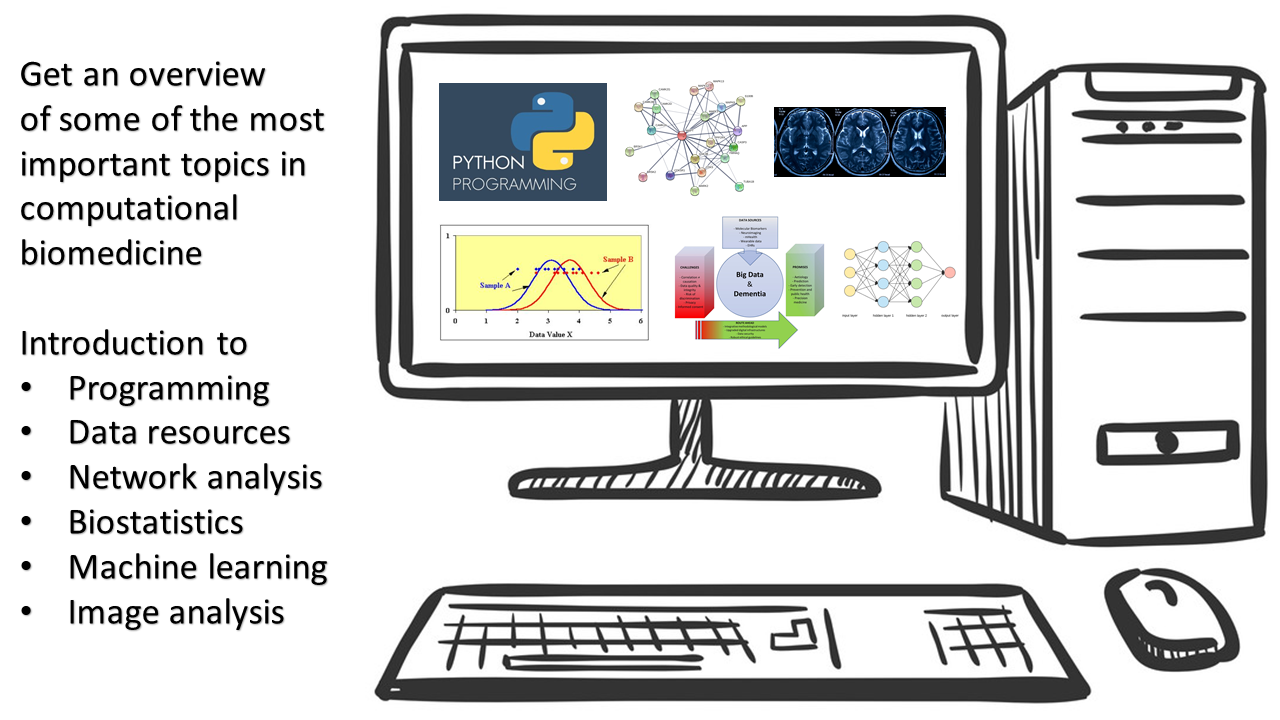
\includegraphics{assets/overview.png}

\hypertarget{learning-objectives}{%
\section{Learning objectives}\label{learning-objectives}}

The aim of the course is to introduce you to important concepts within the field of computational biomedicine as well as to programming. It will provide you with knowledge and ideas that can help you bridge the communication between traditional molecular biologist and computational biologists, and hopefully inspire you to how you can use computational biomedicine in your own research.

This course does not claim to make you an expert within computational science, or train you to do sophisticated programming on your own. These are skills you would need to develop further in follow-up courses or projects. However, we hope that the relevance and practical challenges \& solutions become easier to connect with theory by going over the exercise materials.

\hypertarget{future}{%
\section{Future}\label{future}}

Computational biomedicine is a rapidly growing and evolving field. This is partly due to the changes - or paradigm shift - going on in the fields of cell and molecular biology: a change from a reductionist approach with focus on the biology of a single or a few components to a much more integrative approach where we look at systems biology. This change is highly driven by the development within computer science and large-scale studies in the fields of genomics, proteomics, imaging etc. producing ``big data'' that needs to be integrated in order to obtain relevant and important knowledge within biomedicine. Traditional molecular biology researchers therefore needs to team up with experts within the fields of computational sciences and develop advanced computer algorithms, databases, statistical tools and mathematical models. Such interdisciplinary studies are the way forward for development of e.g.~personalized and predictive medicine and precision diagnostics tools.

\hypertarget{introduction-to-computational-biomedicine-and-machine-learning}{%
\chapter{Introduction to Computational Biomedicine and Machine Learning}\label{introduction-to-computational-biomedicine-and-machine-learning}}

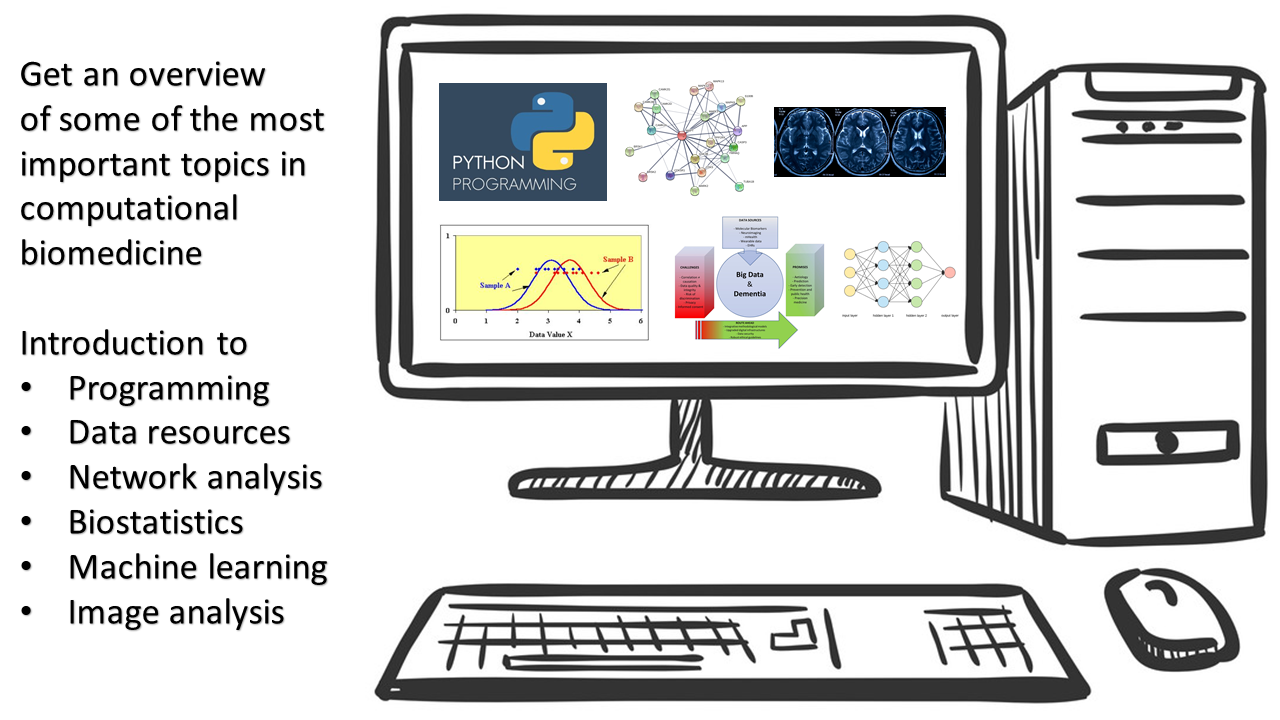
\includegraphics{assets/overview.png}

Short summary

This book accompanies course materials that we share via GitHub. The materials have been put together with the goal to introduce computational biomedicine to students who may enroll to Biomedicine curriculum programs, however we have also used the materials to teach computational students about possibilities of different methods in context of biomedical applications.

The material covers important tools and data resources in this field, and through applications we aim to demonstrate what basic knowledge in network analysis, mathematical models, statistics and machine learning that is needed to work with and understand results from high-throughput biomedical experiments (imaging and omics). For each topic there are hands-on data analysis exercises in Jupyter notebook format and this book is meant to cover some basic background related to each exercise.

\hypertarget{what-is-this-course-about}{%
\section{What is this course about?}\label{what-is-this-course-about}}

The quantitative aspect of biology is inherent to biology, although it is often overlooked. This is because Nature is quantitative. The amount of rain that falls on a particular territory, and not only whether it rains or not, dictates the amount/type of vegetation, which eventually dictates the amount/type of animals the territory can feed.

Lord Kelvin expressed his view in 1883, ``When you can measure what you are speaking about, and express it in numbers, you know something about it;
but when you cannot measure it, when you cannot express it in numbers, your knowledge is of a meager and unsatisfactory kind:
it may be the beginning of knowledge, but you have scarcely, in your thoughts, advanced to the stage of science, whatever the matter may be.''

In this introductory course to computational biomedicine we aim to give you an overview of the different steps related to acquisition, processing, visualization and analysis of quantitative data, and its integration in predictive quantitative models.

\hypertarget{systems-biomedicine}{%
\section{Systems biomedicine}\label{systems-biomedicine}}

Systems biology/biomedicine is a conceptual approach, developed to study biological sciences from a quantitative perspective. It is very recent - the first Institute for Systems Biology was created in 2000 in Seattle by Leroy Hood and coworkers, following the first whole genome sequencing results in the late nineties in unicellular organisms. These groundbreaking datasets revealed the enormous complexity of biological systems: eukaryotic genomes are made of millions, if not billions of base pairs, all of which can virtually affect the functioning of the entire organism.

As nicely explained in this video by Dr.~Leroy Hood, researchers at this time needed a way, a state of mind, to conceptually think of entire biological systems in a more global way, as an alternative to the ``older'' reductionist biology/medicine approach that consists in dissecting the components of the system to find molecular targets to cure diseases.

\hypertarget{new-frontiers---explorers-survival-toolkit}{%
\section{New frontiers - explorer's survival toolkit}\label{new-frontiers---explorers-survival-toolkit}}

The first genome of a human individual was sequenced in 2008. This is just a decade ago. So yes, we are, you are explorers on a brand new mountain route. And every explorer needs a survival toolkit. May this course and similar ones be your toolkits!

Specifically, you will develop skills in systems-level thinking, biological network analysis and quantitative biomedicine. You will learn about important programming tools and the basics of biostatistics and machine learning methods, that you will apply to analyze datasets from your own or from data resources, in order to become able to work with and understand results from high-throughput biomedical experiments (imaging and omics).

\hypertarget{systems-level-thinking}{%
\section{Systems-level thinking}\label{systems-level-thinking}}

Let's understand first why it is very, very important to fully appreciate the added value of quantitative and computational tools to biomedicine.

\hypertarget{networks}{%
\chapter{Networks}\label{networks}}

Let's start by an analogy. Let's envision biological systems as train networks.
Video 1

This is what we talk about in the video:
We will be looking at the train network in Finland. Nodes on this network are city train stations, connected by railways. For a cell biologist, these nodes can be genes, proteins, or other biological molecules, connected by molecular interactions, or even cellular states connected by transitions. For a neurologist, they are neuronal cells, connected by synapses. For an ecologist, these nodes are individual species, connected by trophic predator-prey interactions.

\hypertarget{biological-networks}{%
\section{Biological networks}\label{biological-networks}}

Most if not all the current diseases that challenge our therapeutic abilities have cell biological roots, so let's adopt the point of view of a cell biologist. A cellular function is defined by a particular response to a particular stimulus, multiple stimuli, or the absence of stimulus.

It is analogous to a well-defined travel from, for instance Oulu in the north to Lappeenranta in the south. This trip generally involves a train change in Kouvola. For the cellular function to be performed correctly, the Lappeenranta protein node or cellular state has to be activated in due time.

\hypertarget{disease-from-a-network-perspective}{%
\section{Disease from a network-perspective}\label{disease-from-a-network-perspective}}

Diseases occur when the cellular response to the stimulus is not appropriate, in other words when the travel does not end up where or when it should. For instance, activating the Lahti node instead of the Lappeenranta node could mean activating cell proliferation rather than quiescence, leading to cancer.

On cellular level, diseases perturb how messages are propagated (train travelers) propagate throughout the network. Treating a disease is equivalent to being able to counteract network perturbations, in our train analogy to get to Lappeenranta, regardless of the nature of the perturbations. And if possible, not adding more perturbations.

To treat the Lahti node problem, we could just\ldots{} blow up the Lahti station. This way, no train will ever end up in Lahti, or even transit through the station. This is what we do when we use antiproliferative drugs to treat cancer. And clearly, this certainly affects other travelers, other cellular responses to other stimuli, explaining the toxicity of anticancer agents for instance. In addition, it does not guarantee you will get to Lappeenranta. You could even get to a worse node!

So we definitely need a finer approach, and this requires a deeper knowledge of how the train network works.

\hypertarget{identifying-the-functional-modules}{%
\section{Identifying the functional modules}\label{identifying-the-functional-modules}}

\begin{itemize}
\tightlist
\item
  Do you think that a traveler from Oulu to Lappeenranta needs to know all the timetables of all the Finnish trains to circumvent network perturbations and go to destination?
\end{itemize}

Certainly not. But knowing some key railway routes, hub stations, regional subnetworks and the national lines connecting them, and some late trains timetable will certainly help. And this is what systems biomedicine is about: identifying the cellular functional modules, how they are connected and impinge on one another, in order to understand how to pharmacologically manipulate them in a fine, subtle way.

So let's get back to square one, where our cell is an unknown, mysterious land. With genome sequencing efforts, high-throughput computational analysis of the sequences, and further biochemical characterizations, we have identified tens of thousands of cellular network components, like proteins or mRNAs. This data is in large part openly shared to the scientific community through large data repositories.

This is still work in progress, as we are continuously identifying new network nodes, like for instance recently long non-coding RNAs or small ORFs that code for microproteins of a few residues.

\hypertarget{identifying-interactions}{%
\section{Identifying interactions}\label{identifying-interactions}}

\begin{itemize}
\tightlist
\item
  Do you think knowledge of the train stations is sufficient to travel from Oulu to Lappeenranta?
\end{itemize}

Obviously, not. So, in parallel, scientists are using genetics, biophysical, biochemical, cell biological and many other approaches to characterize the interactions between these nodes, the railway routes. A very common approach is to close one station and look which travels are affected, the knock-out approach, or to shut down one railway line and analyze the resulting perturbations, like for instance when a particular protein-protein interaction is disrupted by a controlled point mutation.

And this is where we stand as per 2020. We are progressively revealing a dense network of interactions between cellular objects, and how well-identified disease-causing mutations modify these interactions. We are therefore learning about finer and finer details of the regional and local train networks, and how these networks are structurally altered in disease.

\hypertarget{network-structure-vs-dynamics}{%
\section{Network structure vs dynamics}\label{network-structure-vs-dynamics}}

Yet we lack ways to efficiently circumvent perturbations on our favorite Oulu Lappeenranta route. And indeed, the more node connections we are revealing, the more it becomes clear that this knowledge is both absolutely required, and at the same time insufficient to predict how to pharmacologically control the response of the network to a given stimulus, or ``information''. Indeed, the knowledge of the network structure, for instance relevant proteins and their interactions, does not tell how it is functionally organized to gather, store and process information and signals {[}1{]}. Knowing the network does not tell us where and when the trains are circulating, how the biological information flows through the network.

And because we are talking about information, let's borrow some concepts from information specialists: the journalists. In journalism, a piece of information is considered complete if it encloses the answers to the 6 W's, 6 basic questions:

\begin{itemize}
\tightlist
\item
  Who? What? When? Where? hoW? and Why?
\end{itemize}

The identification of biological network components answers ``who'' does ``what''. In many instances, the information of when, where and in particular how or how much is missing. As explained in details in the next video, this lack of quantitative information can have a very detrimental effect on our understanding of how a given network works. And this precludes our understanding of the ``why'' biological networks are structured the way they are, and are hijacked by well-identified disease-causing network perturbation. The systems biology, or systems biomedicine approach is aiming to understand biological systems at a global, functional level, in order to decipher their design principles.

And this strategy is particularly relevant in medicine. As different individuals from the same species, we have slightly different genomes, and our cellular networks are a tiny bit different. In addition, we have different lifestyles and even the networks of twins are differentially tuned. Thus, the same disease perturbation in different individuals might have different outcomes, and would thus require slightly adjusted treatments. This observation is at the basis of the concept of personalized medicine.

\begin{itemize}
\tightlist
\item
  Does that mean that any treatment, for any disease must be personalized to be efficient?
\end{itemize}

Absolutely not, because despite their differences, our cellular networks share a lot of functional similarities, emphasizing the importance to understand the functional structure of cell biological networks.

Additional reading:
{[}1{]} Nurse, P. (2008) Life, logic and information. Nature 454, 424--426., and the many positive and negative comments on this article.

\hypertarget{quantitative-biomedicine}{%
\chapter{Quantitative biomedicine}\label{quantitative-biomedicine}}

In this video, we continue with the train station analogy. The purpose of this video is to convince you that this quantitative information is a crucial requirement to understand a biomedical problem, in particular at the systems level.

Video 2

Video content:

The complexity of cell biological diseases stems from the fact that many different molecular events can contribute to the physiological perturbations of the disease state. The diverse disease-associated molecular events apply diverse constraints on the cellular network, resulting in quantitative imbalances in cellular states that call for quantitative approaches.

In most biomedical research fields, the 6 basic questions a journalist would ask are only partially answered. The information of when, where and how much of the cellular components are interacting is missing.

Let us come back to our train network analogy. A critical mutation in the Kouvola station like for instance broken eastbound railways could deviate all trains towards Lahti. But alternatively, delays resulting from railway maintenance works much further north could results in afternoon passengers missing the last eastbound correspondence, leaving no other choice that going westbound or staying in Kouvola. In this situation, however, morning passengers would still be able to proceed to Lappeenranta.

\hypertarget{network-components-vs-parameters}{%
\section{Network components vs parameters}\label{network-components-vs-parameters}}

In the presence of a mutation, the network itself is altered. In the presence of a delay in the signal processing, the network is intact. However a change in a quantitative parameter of the network, a delay in train progression, had the same overall effect for the afternoon travelers, but no effect at all for the morning travelers. Hence, in this case, the way the network responds to the perturbation also depends on the timing of the stimulus. From a therapeutic perspective, pharmacologically restoring the broken railway, or adding late trains from Kouvola to Lappeenranta would be two efficient but radically different ways to solve the disease problem in the two situations.

But choosing between these two strategies would require first to know that Kouvola is a hub connection separating networks in south east from south west finland, in other words a connection separating two functional subnetworks. This is not obvious looking at the network structure only, and systems approaches can help identify these kind of hubs.

Another therapeutic strategy that would work in both situations could be to re-route our train way upstream of the Kouvola hub region, through Eastern Finland. Again, the pharmacological implementation of this strategy would require an a priori knowledge of how the northern, eastern and southeastern subnetworks communicate. Moreover, this strategy should be supplemented with additional east-west trains to compensate for the loss of the Oulu-Kouvola connection.

Beyond spatial and temporal parameters, ``how much'' cellular components are present and interact can have a drastic effect on the network response to the stimulus. Assume that in the normal cell, the conductor of the Oulu-Kouvola train changes at the Pieksämäki station, with a new conductor coming from Joensuu and the original one leaving on a train to south west Finland. Assume a sick cell has delays in conveying the second conductor to pieksämäki, then the first one is left with three options: wait, leading to delays at Kouvola, as discussed a minute ago. Keep on its original schedule, leaving our train in Pieksämäki; or carry on, leading to the cancelation of the westbound train. In this scenario, the number of train conductors available in Pieksämäki becomes a limiting factor due to the disease-associated quantitative delays, forcing the cell to make a decision between three choices that will all have detrimental consequences.

Train staff is regularly transported by trains, and these situations are common in train network management. But because the decisional units at the headquarters of the train company have all the information on the current status of the network in hand, and know all the scheduled trains, they can make a wise decision to fix the problem.

In biomedicine, because we don't have all this quantitative information, we can't. In addition, our lack of quantitative knowledge might also confound our analysis of the network structure itself: in the last example, because train conductors are nearly limiting in the normal cell, a perturbation on the Joensuu-Pieksämäki axis shows strong effects on a completely different line. Hence, it might give the impression to the unprepared experimentalist that the Joensuu-Pieksämäki axis is literally on the Oulu Kouvola axis. In fact it is not, but the limitation in the number of train conductors generates an effective strong connection between the Eastern Finland network and the north south axis.

Hence, this naïve analogy between biological and train networks teaches us that it is crucial to learn more about quantitative parameters of the biological networks, in order to devise clever therapeutic strategies that shall target the regulation of multiple distinct functional modules at the systems level. Once we are able to know how many trains take which routes, when, who are the passengers, conductors\ldots{} and so on and so forth, then we will be able to devise efficient therapeutic strategies, certainly involving synchronized regulation of multiple, well-chosen targets and functions. Along the same lines, we recommend reading Yuri Lazebnik's paper ``Can a biologist fix a radio? Or, what I learned while studying apoptosis'', published 20 years ago but still very relevant today {[}2{]}.

Additional reading:
{[}2{]} Lazebnik Y. (2002) Can a biologist fix a radio? Or, what I learned while studying apoptosis. Cancer Cell 2:179-82, and the comments on this article.

\hypertarget{language-barriers}{%
\chapter{Language barriers}\label{language-barriers}}

\hypertarget{descriptive-language---qualitative}{%
\section{Descriptive language - qualitative}\label{descriptive-language---qualitative}}

Biomedical systems are made of cells, cells of molecules, molecules of atoms \ldots etc. The biology language has been developed over centuries to describe macroscopic biological systems, mostly at the qualitative level.

\hypertarget{quantitative-language}{%
\section{Quantitative language}\label{quantitative-language}}

Physics is an example of a quantitative language which can describe molecules, and to describe atoms. In quantum physics the langueage is that of mathematics.

These language differences stem from the historical distinction between life sciences and physical sciences, and we are now realizing that this distinction does not make a lot of sense.

\hypertarget{programming-languages}{%
\section{Programming languages}\label{programming-languages}}

Furthermore, you are using also another type of language, programming, to write down the analysis steps in a computer-understandable format, because most biological problems cannot be solved by current analytical mathematics.

\hypertarget{interdisciplinary-science}{%
\section{Interdisciplinary science}\label{interdisciplinary-science}}

When you are working on the quantitative analysis of cells - which is what you want to do for doing predictive biomedicine - you are at the crossroads of these languages, all of which have advantages and pitfalls.

There is not, yet, any common language perfectly suited to quantitative cell biology or systems-level medicine that would be understood by experts of all these fields. Therefore, inter-disciplinary communication will require that biologists learn the basic concepts and formal language of quantitative sciences and basic programming skills, and that physicists or mathematicians eager to contribute in transforming future medicine learn some elementary cell and molecular biology concepts. This will enable you to collaborate and communicate with a broad range of specialists, physicists, mathematicians, computer scientists, geneticists, biochemists\ldots{} etc.

Another current challenge in this field is related to what data and tools are available to the community at large (Macklin 2019) . It is an important goal to move beyond single-laboratory efforts to establish a community dedicated to promote compatible data and software usage.

\hypertarget{intro}{%
\chapter{How to contribute to the book}\label{intro}}

\hypertarget{r-markdown-instructions-from-bookdown-example}{%
\section{R markdown instructions from bookdown example:}\label{r-markdown-instructions-from-bookdown-example}}

You can label chapter and section titles using \texttt{\{\#label\}} after them, e.g., we can reference Chapter \ref{intro}. If you do not manually label them, there will be automatic labels anyway, e.g., Chapter \ref{methods}.

Figures and tables with captions will be placed in \texttt{figure} and \texttt{table} environments, respectively.

\begin{Shaded}
\begin{Highlighting}[]
\FunctionTok{par}\NormalTok{(}\AttributeTok{mar =} \FunctionTok{c}\NormalTok{(}\DecValTok{4}\NormalTok{, }\DecValTok{4}\NormalTok{, .}\DecValTok{1}\NormalTok{, .}\DecValTok{1}\NormalTok{))}
\FunctionTok{plot}\NormalTok{(pressure, }\AttributeTok{type =} \StringTok{\textquotesingle{}b\textquotesingle{}}\NormalTok{, }\AttributeTok{pch =} \DecValTok{19}\NormalTok{)}
\end{Highlighting}
\end{Shaded}

\begin{figure}

{\centering 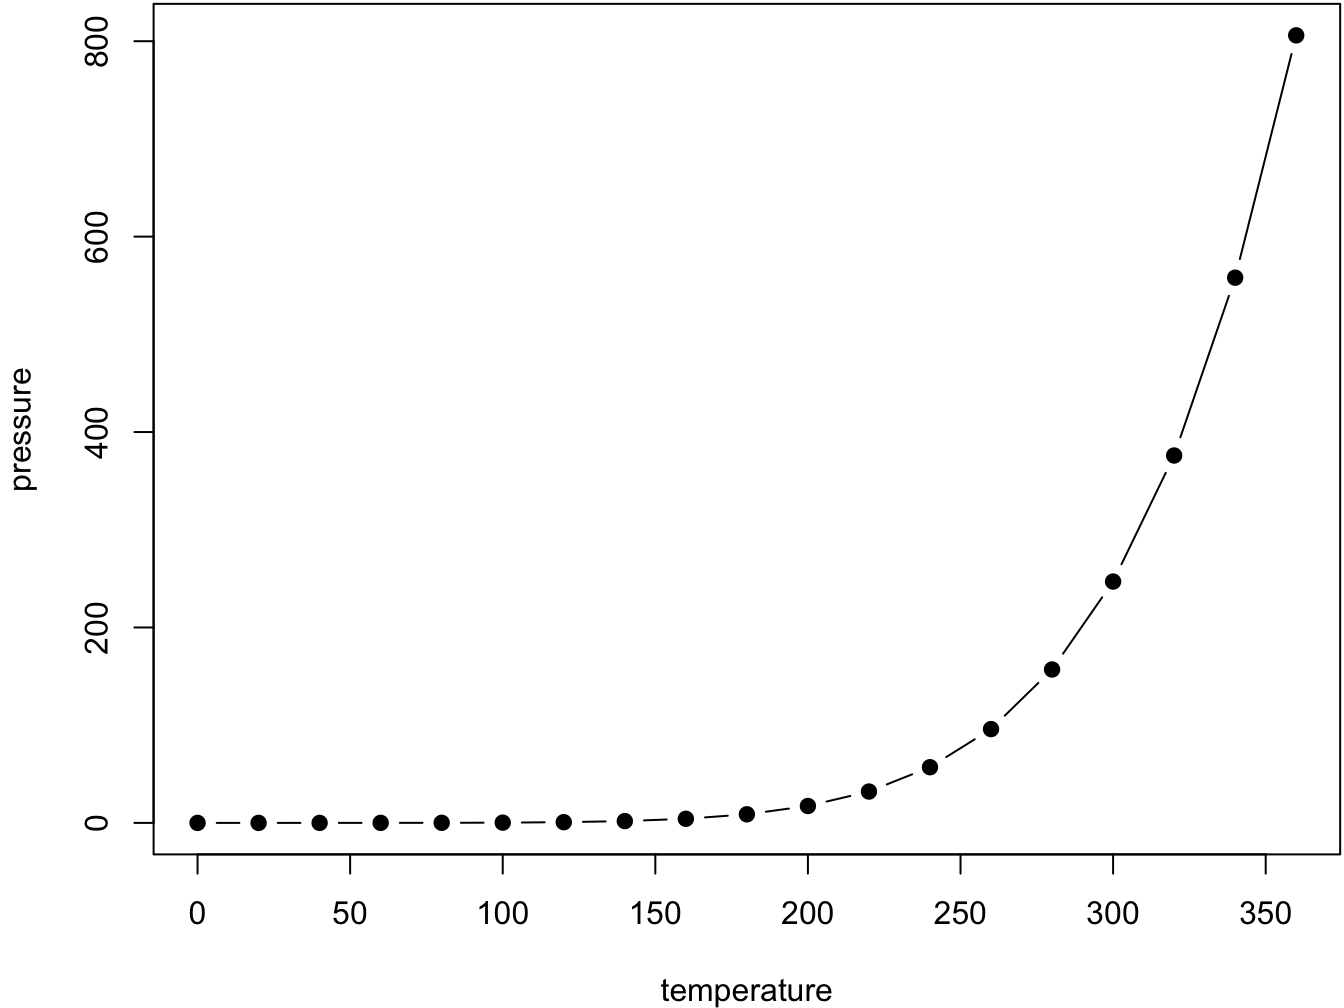
\includegraphics[width=0.8\linewidth]{testBook_files/figure-latex/nice-fig-1} 

}

\caption{Here is a nice figure!}\label{fig:nice-fig}
\end{figure}

Reference a figure by its code chunk label with the \texttt{fig:} prefix, e.g., see Figure \ref{fig:nice-fig}. Similarly, you can reference tables generated from \texttt{knitr::kable()}, e.g., see Table \ref{tab:nice-tab}.

\begin{Shaded}
\begin{Highlighting}[]
\NormalTok{knitr}\SpecialCharTok{::}\FunctionTok{kable}\NormalTok{(}
  \FunctionTok{head}\NormalTok{(iris, }\DecValTok{20}\NormalTok{), }\AttributeTok{caption =} \StringTok{\textquotesingle{}Here is a nice table!\textquotesingle{}}\NormalTok{,}
  \AttributeTok{booktabs =} \ConstantTok{TRUE}
\NormalTok{)}
\end{Highlighting}
\end{Shaded}

\begin{table}

\caption{\label{tab:nice-tab}Here is a nice table!}
\centering
\begin{tabular}[t]{rrrrl}
\toprule
Sepal.Length & Sepal.Width & Petal.Length & Petal.Width & Species\\
\midrule
5.1 & 3.5 & 1.4 & 0.2 & setosa\\
4.9 & 3.0 & 1.4 & 0.2 & setosa\\
4.7 & 3.2 & 1.3 & 0.2 & setosa\\
4.6 & 3.1 & 1.5 & 0.2 & setosa\\
5.0 & 3.6 & 1.4 & 0.2 & setosa\\
\addlinespace
5.4 & 3.9 & 1.7 & 0.4 & setosa\\
4.6 & 3.4 & 1.4 & 0.3 & setosa\\
5.0 & 3.4 & 1.5 & 0.2 & setosa\\
4.4 & 2.9 & 1.4 & 0.2 & setosa\\
4.9 & 3.1 & 1.5 & 0.1 & setosa\\
\addlinespace
5.4 & 3.7 & 1.5 & 0.2 & setosa\\
4.8 & 3.4 & 1.6 & 0.2 & setosa\\
4.8 & 3.0 & 1.4 & 0.1 & setosa\\
4.3 & 3.0 & 1.1 & 0.1 & setosa\\
5.8 & 4.0 & 1.2 & 0.2 & setosa\\
\addlinespace
5.7 & 4.4 & 1.5 & 0.4 & setosa\\
5.4 & 3.9 & 1.3 & 0.4 & setosa\\
5.1 & 3.5 & 1.4 & 0.3 & setosa\\
5.7 & 3.8 & 1.7 & 0.3 & setosa\\
5.1 & 3.8 & 1.5 & 0.3 & setosa\\
\bottomrule
\end{tabular}
\end{table}

You can write citations, too. For example, we are using the \textbf{bookdown} package \citep{R-bookdown} in this sample book, which was built on top of R Markdown and \textbf{knitr} \citep{xie2015}.

  \bibliography{book.bib,packages.bib}

\end{document}
